\section{Zielsetzung}
\label{sec:Zielsetzung}
In diesem Versuch soll die Funktionsweise eines Lock-In-Verstärkers untersucht werden.

\section{Theorie}
\label{sec:Theorie}
Ein Lock-In-Verstärker (schematischer Aufbau: s. Abb \ref{fig:aufbau}) ist ein Verstärker mit eingebautem phasenempfindlichen Detektor. Dieser dient bei der Messung stark verrauschter Signale als extrem 
schmalbandiger Bandpassfilter, wodurch das Rauschen effizient gefiltert werden kann. Das Messsignal kann dazu mit einer Referenzfrequenz $\omega_{0}$ moduliert werden.

Der Bandpassfilter befreit das modulierte, verrausche Nutzsignal $U_{\text{sig}}$ von Rauschanteilen höherer ($\omega \gg \omega_{0} $) und niedrigerer Frequenzen ($\omega \ll \omega_{0}$).
Als nächstes wird das Nutzsignal $U_{\text{sig}}$ mit dem Referenzsignal $U_{\text{ref}}$ multipliziert, welches eine variable Phase besitzt.
Mit einem Phasenschieber wird die Phase des Referenzsignals vor dem Mischer variiert, um sie mit der Phase des verrauschten Signals synchronisieren zu können. Als Ergebnis folgt dann ein 
Tiefpass ($\tau = RC \gg \frac{1}{\omega_{0}}$), welcher das multiplizierte Mischsignal integrieren kann, damit die Rauschbeiträge herausgemittelt werden können. 

Es ergibt sich eine proportionale Gleichspannung zur Eingangsspannung für das Signal:
\begin{equation*}
U_{\text{out}} \propto U_{0}cos(\phi)
\end{equation*}
wobei $\phi$ die Phasenlage zwischen den beiden Signalen ist. 

\begin{figure}[h!]
	\centering
	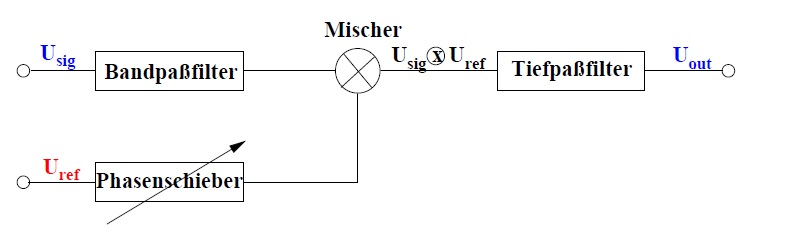
\includegraphics[width=0.8\linewidth]{Aufbau.jpg}
	\caption{Schematischer Aufbau des Lock-In-Verstärkers. \cite[1]{anleitung303}}
	\label{fig:aufbau}
\end{figure}

Der Tiefpass definiert also die Bandbreite des Restrauschens:
\begin{equation*}
\Delta \nu = \frac{1}{\pi RC}.
\end{equation*}
Dies gilt nur in dem Fall, wenn die Zeitkonstante $\tau = RC$ sehr groß gewählt wird, damit die Bandbreite belieblig klein gehalten werden kann. 

\subsection{Sinusspannung}
Als Beispiel wird eine sinusförmige Spannung in der Abbildung \eqref{fig:sinus} betrachtet. Sie ist gegeben als: 
\begin{equation*}
U_{\text{sig}} = U_{0}sin(\omega t).
\end{equation*}

\begin{figure}[h!]
	\centering
	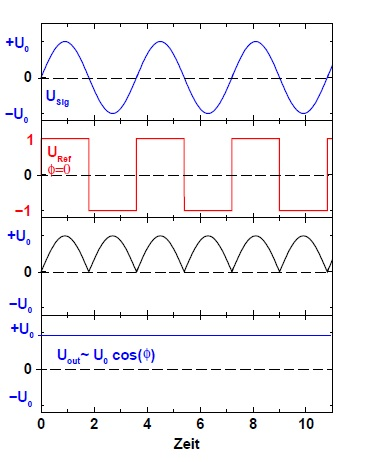
\includegraphics[width=0.7\linewidth]{sinus.jpg}
	\caption{Die Signalverläufe der sinusförmigen Signalspannung: Sinusspannung(1), Referenzspannung(2), gemischte Signale(3), Ausgabesignal des Tiefpasses(4). \cite[2]{anleitung303}}
	\label{fig:sinus}
\end{figure}

Es wird eine Referenzsignal verwendet, welches in diesem Fall eine Rechteckspannung mit einer auf $1$ normierten Amplitude enthält. Sie kann durch die Fourier-Reihe angenähert werden:
\begin{equation*}
U_{\text{ref}} = \frac{4}{\pi} \left(\text{sin}(\omega t) + \frac{1}{3}\text{sin}(3\omega t) + \frac{1}{5}\text{sin}(5\omega t) + ... \right).
\end{equation*}
Für das Produkt der beiden Signale ergibt sich:
\begin{equation*}
U_{\text{sig}} \times U_{\text{ref}} = \frac{2}{\pi}U_{0} \left(1 - \frac{2}{3}\text{cos}(2 \omega t) - \frac{2}{15}\text{cos}(4 \omega t) - \frac{2}{35}\text{cos}(6 \omega t) + ... \right),
\end{equation*}
wobei dieses dann die gerade Oberwelle der Grundfrequenz $\omega$ entspricht (s. Abbildung \ref{fig:sinus}).

Der Tiefpass wird dann im folgenden so gewählt, dass die Oberwellen unterdrückt werden und sich somit eine zur Signalspannung proportionale Gleichspannung ergibt:
\begin{equation*}
U_{\text{out}} = \frac{2}{\pi}U_{0}\text{cos}(\phi).
\end{equation*}
Die höchste Ausgangsspannung ergibt sich bei einer Phasendifferenz der beiden Signale von $\phi = 0 $.